% !TeX program = xelatex

\documentclass[landscape,twocolumn,a5paper]{manual}
\usepackage[margin=0.33in,bottom=0.5in,footskip=0.25in]{geometry}

\definecolor{themered}{HTML}{8B3232}
\colorlet{theme}{themered}

\pluginname{ChowTape}

\def\pluginfolder{\href{https://help.uaudio.com/hc/en-us/articles/210216306-Default-Install-Locations-for-UAD-Plug-Ins}{plugin folder}}
\def\dllink#1{\href{https://github.com/jatinchowdhury18/AnalogTapeModel/releases}{#1}}

\begin{document}

\section{ChowTape User Manual}

\noindent
\boldtheme{ChowTape} is an analog tape machine physical model,
originally based on the Sony TC-260. The current version
can be used to emulate a wide variety of reel-to-reel tape
machines. As well as a tool for mixing engineers and producers,
ChowTape is a research project on developing physics-based
models of analog tape emulation\footnote{The plugin is based off a 2019 DAFx paper
\href{http://dafx2019.bcu.ac.uk/papers/DAFx2019_paper_3.pdf}{``Real-time Physical Modelling for Analog Tape Machines''}.}.
The plugin is currently available as VST/VST3/AU/LV2 for
Windows, Linux, and Mac.

\subsection{Installation}
To install ChowTape for Mac or Windows, download the
\dllink{latest release}, unzip the downloaded file, and copy
the plugin files to your \pluginfolder. Note that Macintosh
users may need to
\href{https://www.imore.com/how-open-apps-anywhere-macos-catalina-and-mojave}{allow applications from unidentified developers}.
Linux users may download builds from the
\href{https://build.opensuse.org/package/show/home:kill_it:JUCE/CHOWTapeModel}{Open Build Service}, or
\href{https://github.com/jatinchowdhury18/AnalogTapeModel/blob/master/BUILDING.md}{compile from source}.

\begin{figure}[ht]
    \center
    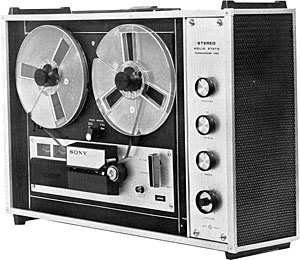
\includegraphics[width=0.55\columnwidth]{../Refs/Pictures/sony_tc-260.jpg}
    \caption{\label{TapeMachine}{\it A Sony TC 260 reel-to-reel tape machine}}
\end{figure}

% @TODO: figures for controls...

\subsection{Controls}
ChowTape contains a wide range of controls allowing the
user to design the the physical characteristics of the tape
machine and magnetic tape being emulated. Several of the
controls even allow the user to achieve more ``extreme''
results than would be possible with a physical tape machine.

\subsubsection{Main Controls}
\boldtheme{Input Gain} controls the gain level going into the
rest of the plugin. Note that abnormally large levels can
cause the plugin to become unstable, so it is recommended
that your levels are below unity gain going into the plugin,
and any extra gain you wish to add should come from the input
gain control. %@TODO: more notes on stability
\newpar
\boldtheme{Dry/Wet} allows the user to choose how much of the
signal they want to the plugin's processing to affect.
\newpar
\boldtheme{Output Gain} controls the level coming out of the plugin.
\newpar
\boldtheme{Oversampling} controls the amount of oversampling
being done internally within the plugin. More oversampling
will result in a higher quality sound with fewer aliasing
artifacts and better noise characteristics, but will also
use more of your CPU. It is recommended to use as much
oversampling as your CPU will allow.
\newpar
\boldtheme{Mix Group}: When using ChowTape on multiple channels
in your mix, you can synchronize parameters between plugin
instances belonging to the same mix group. Essentially, all
the plugin instances in the same mix group will share the same
parameters.

\subsubsection{Hysteresis Controls}
@TODO
\boldtheme{Hysteresis Mode}
\boldtheme{Drive}
\boldtheme{Saturation}
\boldtheme{Bias}

\subsubsection{Tone Controls}
The tone section applies a set of pre-/post-emphasis filters
to the signal before and after the hysteresis processing
is applied. The filters work similar to
\href{https://en.wikipedia.org/wiki/RIAA_equalization}{RIAA filters},
in that the pre- and post- filters have exact opposite frequency
responses.
\newpar
The \boldtheme{Bass} and \boldtheme{Treble} knobs control
the frequency response of the pre-emphasis filter, and the
post-emphasis filter will automatically adjust. The
\boldtheme{Frequency} knob controls the transition frequency
between the bass and treble sections of the filter.

\subsubsection{Playhead Controls}
Physical tape machines also have a frequency response that
is affected by the amount of space between the playhead and
the tape, the width of the playhead gap, and the thickness
of tape used. The frequency responses of each of these ``loss
effects'' is also dependent on the tape speed.
\newpar
\boldtheme{Spacing}
controls the amount of space between the playhead and the tape,
measured in centiimeters.
\newpar
\boldtheme{Thickness} controls the thickness
of the tape, measured in centiimeters.
\newpar
\boldtheme{Gap} controls
the width of the playhead gap, measured in millimeters.
\newpar
\boldtheme{Speed}
controls the tape speed as it effects the above loss effects,
measured in inches per second (ips). While this control is
continuous, standard tape speeds are 7.5, 15, and 30 ips.

\subsubsection{Tape Degradation Controls}
The degradation parameters control a simulation of old, degraded
tape.
\newpar
\boldtheme{Depth} and \boldtheme{Amount} control the amount of
degradation that is added to the tape, while \boldtheme{Variance}
adds a time-varying randomness to the degradatation.

\subsubsection{Chew Controls}
The chew parameters simulate tape that has been chewed up by
a broken tape machine.
\newpar
\boldtheme{Depth} controls how deep the tape is chewed;
\newpar
\boldtheme{Frequency} controls how much space there is between
bits of tape that have been chewed up.

\subsubsection{Wow and Flutter Controls}
Tape machines also exhibit timing irregularities, often due
to small imperfections in the mechanics of the machine causing
the tape to subtly speed up and slow down while being
played back. The flutter characteristic in this plugin was
measured from an original Sony TC-260 tape machine.
\newpar
\boldtheme{Rate} controls the rate of flutter, with higher values
causing the flutter to occur faster.
\newpar
\boldtheme{Depth} controls the depth of the flutter, with 0 meaning
that no flutter is occuring, and higher values making the flutter
more noticeable.
\newpar
"\boldtheme{Wow}" is similar to flutter but on a much longer time scale,
and contains similar controls.


\end{document}
